% Options for packages loaded elsewhere
\PassOptionsToPackage{unicode}{hyperref}
\PassOptionsToPackage{hyphens}{url}
%
\documentclass[
]{article}
\usepackage{amsmath,amssymb}
\usepackage{lmodern}
\usepackage{iftex}
\ifPDFTeX
  \usepackage[T1]{fontenc}
  \usepackage[utf8]{inputenc}
  \usepackage{textcomp} % provide euro and other symbols
\else % if luatex or xetex
  \usepackage{unicode-math}
  \defaultfontfeatures{Scale=MatchLowercase}
  \defaultfontfeatures[\rmfamily]{Ligatures=TeX,Scale=1}
\fi
% Use upquote if available, for straight quotes in verbatim environments
\IfFileExists{upquote.sty}{\usepackage{upquote}}{}
\IfFileExists{microtype.sty}{% use microtype if available
  \usepackage[]{microtype}
  \UseMicrotypeSet[protrusion]{basicmath} % disable protrusion for tt fonts
}{}
\makeatletter
\@ifundefined{KOMAClassName}{% if non-KOMA class
  \IfFileExists{parskip.sty}{%
    \usepackage{parskip}
  }{% else
    \setlength{\parindent}{0pt}
    \setlength{\parskip}{6pt plus 2pt minus 1pt}}
}{% if KOMA class
  \KOMAoptions{parskip=half}}
\makeatother
\usepackage{xcolor}
\IfFileExists{xurl.sty}{\usepackage{xurl}}{} % add URL line breaks if available
\IfFileExists{bookmark.sty}{\usepackage{bookmark}}{\usepackage{hyperref}}
\hypersetup{
  pdftitle={Proteome wide screen for RNA-dependent Proteins in interphasic HeLa cells},
  pdfauthor={Bolz, C., Bonsen, M., Pott, M., Simon, M.},
  hidelinks,
  pdfcreator={LaTeX via pandoc}}
\urlstyle{same} % disable monospaced font for URLs
\usepackage[margin=1in]{geometry}
\usepackage{graphicx}
\makeatletter
\def\maxwidth{\ifdim\Gin@nat@width>\linewidth\linewidth\else\Gin@nat@width\fi}
\def\maxheight{\ifdim\Gin@nat@height>\textheight\textheight\else\Gin@nat@height\fi}
\makeatother
% Scale images if necessary, so that they will not overflow the page
% margins by default, and it is still possible to overwrite the defaults
% using explicit options in \includegraphics[width, height, ...]{}
\setkeys{Gin}{width=\maxwidth,height=\maxheight,keepaspectratio}
% Set default figure placement to htbp
\makeatletter
\def\fps@figure{htbp}
\makeatother
\setlength{\emergencystretch}{3em} % prevent overfull lines
\providecommand{\tightlist}{%
  \setlength{\itemsep}{0pt}\setlength{\parskip}{0pt}}
\setcounter{secnumdepth}{-\maxdimen} % remove section numbering
\ifLuaTeX
  \usepackage{selnolig}  % disable illegal ligatures
\fi

\title{Proteome wide screen for RNA-dependent Proteins in interphasic
HeLa cells}
\author{Bolz, C., Bonsen, M., Pott, M., Simon, M.}
\date{2022-07-15}

\begin{document}
\maketitle

\hypertarget{introduction}{%
\section{Introduction}\label{introduction}}

RNA and proteins represent a symbiotic system. Proteins need RNA as a
template for their biosynthesis as stated by Francis Crick in his
``Central Dogma of Molecular Biology'' (Crick, 1970). Furthermore,
studies have shown that proteins need RNA for their catalytic activity
for example in the RNA-induced silencing complex (Pratt and Macrae,
2009; Wilson and Doudna, 2013). On the other hand some RNAs depend on
Proteins for their synthesis and stability (Kishore \emph{et al.},
2010). A family of proteins which describe this symbiotic relationship
are RNA-binding proteins (RBPs). RBPs describe a class of proteins whose
interactome depends on RNA and have shown to play a crucial role in RNA
metabolism (Kishore \emph{et al.}, 2010), cancer development (Wei
\emph{et al.}, 2022) and genetic disease (Gebauer \emph{et al.}, 2021).
Therefore a deeper understanding of the mechanisms of RNA binding and
RNA-Protein interaction enhances our ability to regulate and modulate
these processes.

RBPs can be further categorised in ``true'' RBPs (e.g.~DICER, NPM3),
RNA-binding proteins which directly bind to RNAs and ``RBP interacting
proteins'' which interact with ``true'' RBPs (eg. RBBP7). Furthermore
``true RBPs'' can be subcategorized in ``RNA-dependent'', relying on RNA
for their full and correct function (eg. DICER) and ``partially RNA
dependent'', only requiring RNAs for certain functions or transport (eg.
NPM3) (see Fig. 1) (Caudron-Herger \emph{et al.}, 2019; Corley \emph{et
al.}, 2020).

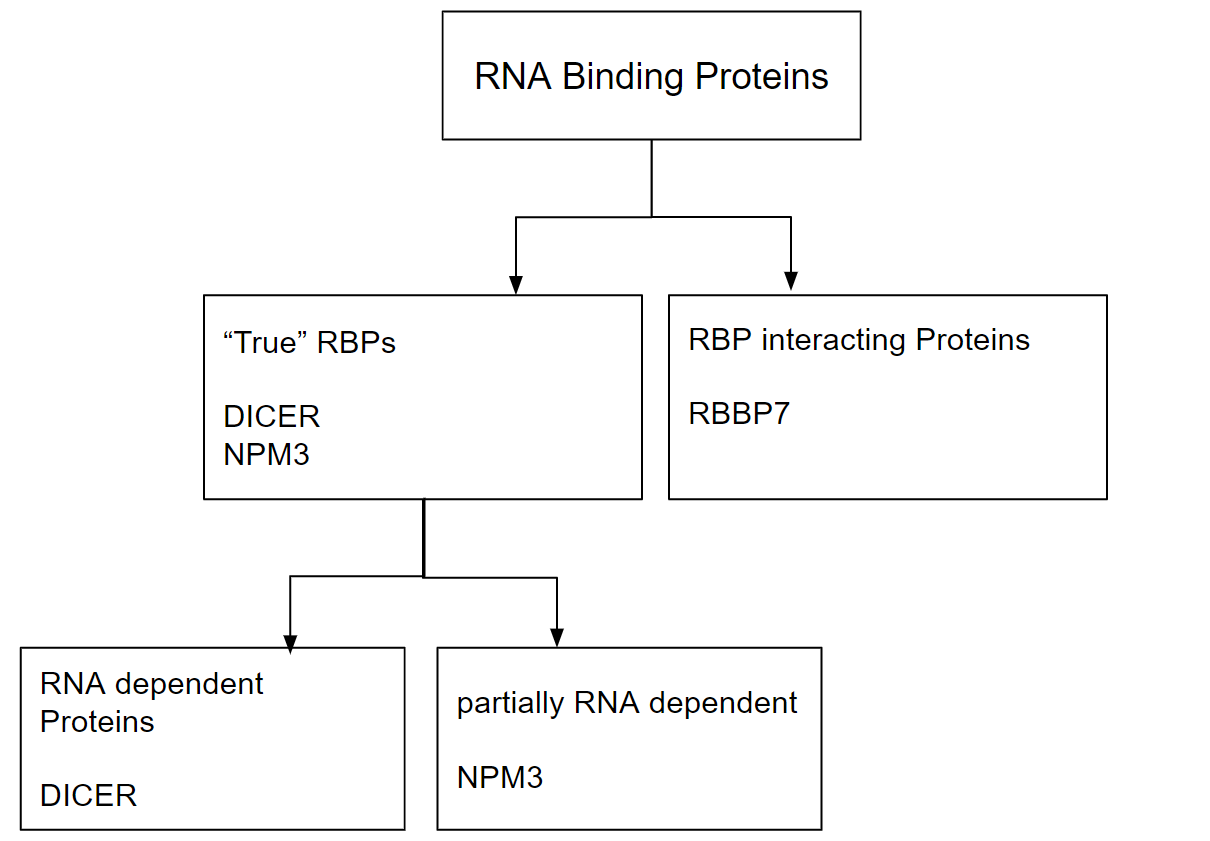
\includegraphics{../../Figure1.PNG}

\textbf{Figure 1}. Categorization of RNA-binding proteins: RBPs can be
categorised in ``true'' RBPs, RNA-binding proteins which directly bind
to RNAs, ``RBP interacting proteins'' which interact with ``true'' RBPs.
``True'' RBPs are subcategorized as ``RNA-dependent'' relying on RNA for
their full and correct function and ``partially RNA dependent'' only
requiring RNAs for certain functions or transport. DICER =
Endoribonuclease Dicer; NPM3 = Nucleoplasmin 3; RBBP7 = RNA-binding
protein binding protein 7.

Several approaches to study RNA-Protein interaction and to identify new
RBPs have been established such as RaPID and CLIP-Seq. These methods
only allow to analyse the interaction between RNA of interest and
proteins (RaPID) or a protein of interest and the RNAs it is interacting
with (CLIP-Seq) (Qin \emph{et al.}, 2021). Therefore several global
approaches have been made to study RNA-Binding Protein interaction
networks (Sternburg and Karginov, 2020). A method published by
Caudron-Herger \emph{et al.} enables analysis and quantification of
whole cell interactomes and identification of new RBPs through RNase
treatment and density gradient ultracentrifugation. This is followed by
a bioinformatic analysis of fraction shifts from proteins identified
with mass spectrometry (Caudron-Herger \emph{et al.}, 2019,
Caudron-Herger \emph{et al.}, 2020).

In this study we analysed a dataset of interphase synchronised HeLa S3
cells obtained by the method published by Caudron-Herger \emph{et al.}
Our aim is to identify, analyse and classify RBPs and possible RBP
candidates using bioinformatical methods in R and cross-referencing with
established databases such as R-DeeP (\url{https://r-deep.dkfz.de/};
Caudron Herger \emph{et al.}, 2019), UniProt
(\url{https://www.uniprot.org/}) and RBP2GO
(\url{https://rbp2go.dkfz.de/}; Caudron-Herger \emph{et al.}, 2021).

\newpage

\hypertarget{methods}{%
\section{Methods}\label{methods}}

\hypertarget{generation-of-the-dataset}{%
\subsection{Generation of the dataset}\label{generation-of-the-dataset}}

Interphasic HeLa S3 cells were harvested and lysed. The lysate was split
into two samples and one sample was treated with an RNase mixture
(referred to as RNase (RNA)) the other sample was left untreated
(referred to as control (ctrl)). Both samples were loaded on a 5 \% to
25 \% sucrose density gradient grouped in 25 fractions and separated
using ultracentrifugation. For each condition technical triplicates were
generated. Each fraction was then analysed using mass spectrometry.
Proteins were identified using UniProt and the amount of protein per
fraction, condition and replicate was stored in arbitrary units in an
.csv-file (for full protocol see: Caudron-Herger \emph{et al.}, 2019). A

\hypertarget{clean-up-and-sorting-of-the-dataset}{%
\subsection{Clean-Up and sorting of the
dataset}\label{clean-up-and-sorting-of-the-dataset}}

Using the R package tidyverse two seperate dataframes were generated
containing either all untreated (\_ctrl) or RNAse treated (\_RNA)
replicates. Both data frames as well as the raw dataset were screened
for rows containing only zeros. Identified rows were removed from the
data frame and stored in a different data frame.

\hypertarget{normalization}{%
\subsection{Normalization}\label{normalization}}

To rule out batch to batch effects and technical errors the protein
amount per replicate (Rep) and fraction (Frac) as well as for each
protein in each condition needs to be normalized.

\hypertarget{fraction-wise-normalization}{%
\subsubsection{Fraction-wise
normalization}\label{fraction-wise-normalization}}

Normaliziation for each fraction was done using the following equation:

\[Protein(Norm) = \frac{maxcolsums}{Colsumme} * Protein(before)\]

\emph{Protein(Norm)} describes the normalized amount of a single protein
per fraction and replicate. \emph{maxcolsums} is the selected maximum
total protein amount per fraction and replicate. For each Fraction one
maxium was chosen. \emph{Colsumme} represents the total amount of
protein per Fraction and replicate. The Parameter \emph{Protein(before)}
describes the amount of a single protein per fraction and replicate
prior to normalization.

\hypertarget{sacling-the-protein-distrubition-per-replicate-and-condition-to-100}{%
\subsubsection{Sacling the protein distrubition per replicate and
condition to
100}\label{sacling-the-protein-distrubition-per-replicate-and-condition-to-100}}

For better comparability of the protein amount per fraction was
displayed as relative using the following equation:

\[Protein(Relative) = \frac{Protein(Frac)}{Protein(Total\ per\ Rep)}*100\]

\emph{Protein(Relative)} describes the relative protein amount per
fraction on relation to the total amount of the protein per replicate.
\emph{Protein(Frac)} represents the amount of a protein per fraction and
replicate. Total amount of protein per Replicate is given by \emph{Total
per Rep}.

\hypertarget{create-separate-dataframes}{%
\subsubsection{Create separate
dataframes}\label{create-separate-dataframes}}

Dataframes for each individual fraction and condition were created,
containing the triplicate values for each protein.

They follow the naming convention:

\begin{enumerate}
\def\labelenumi{\arabic{enumi}.}
\item
  Fraction1\_Ctrl for the triplicate values of first fraction of the
  control group
\item
  Fraction\_8\_RNAse for the triplicate values of eighth fraction of the
  RNase treated sample
\end{enumerate}

\hypertarget{calculation-of-means-and-standard-deviation}{%
\subsection{Calculation of Means and standard
deviation}\label{calculation-of-means-and-standard-deviation}}

Mean and standard deviation for each protein in each fraction was
calculated using the built-in functions \emph{mean()-}(\(\overline x\))
and \emph{sd()-function}\((\sigma)\) of R. Outliers were detected using
\(\overline x \pm 3\sigma\) as cut-off. All values below and above were
replaced with NA and not accounted in following calculations.

\hypertarget{shapiro-wilk-test}{%
\subsection{Shapiro-Wilk Test}\label{shapiro-wilk-test}}

To test for normal distribution Shapiro-Wilk Test is chosen due to its
high power in small populations in comparison to other tests. The test
is performed using an built-in R function \emph{shapiro\_test()}.

\hypertarget{determination-of-maxima}{%
\subsection{Determination of Maxima}\label{determination-of-maxima}}

For all proteins in the control group and treated with RNase the global
and local maxima were determined For this purpose, the protein content
(y-value) was compared to two neighbors right and left of the analyzed
fraction (x-position). As relevant local maxima only those maxima were
selceted that contained more than 2 \% of the protein.

\hypertarget{detection-of-protein-shifts}{%
\subsection{Detection of Protein
Shifts}\label{detection-of-protein-shifts}}

As previous publisehd only peaks

\end{document}
